\section{Sở GD\&ĐT Thái Nguyên 25--26, Lần 1}
\caulc
\Opensolutionfile{ans}[ans/ans-26-2--SoGDThaiNguyen-L1-LC]
\begin{ex}%[Đề thi thử THPT 2026 - SGD Thái Nguyên - Lần 1, Đoàn Hùng]%[1D6N4-4]
	Nghiệm của phương trình $3^{x+1} = 9$ là
	\choice
	{\True $x=1$}
	{$x=4$}
	{$x=3$}
	{$x=2$}
	\loigiai{
		Ta có $3^{x+1} = 9 \Leftrightarrow 3^{x+1} = 3^2 \Leftrightarrow x+1 = 2 \Leftrightarrow x = 1$.\\
		Vậy phương trình đã cho có nghệm duy nhất $x=1$.
	}
\end{ex}

\begin{ex}%[Đề thi thử THPT 2026 - SGD Thái Nguyên - Lần 1, Đoàn Hùng]%[2D1N4-1]
	Tiệm cận đứng của đồ thị hàm số $y = \dfrac{3x-5}{x-2}$ là đường thẳng có phương trình
	\choice
	{$x = \dfrac{3}{5}$}
	{$x = 3$}
	{$x = \dfrac{5}{3}$}
	{\True $x = 2$}
	\loigiai{
		Tập xác định $\mathscr{D}=\mathbb{R}\setminus \{2\}$.\\
		Ta có $\lim \limits_{x \to 2^+} \dfrac{3x-5}{x-2}=+\infty$ và $\lim \limits_{x \to 2^-} \dfrac{3x-5}{x-2}=-\infty$.\\
		Suy ra $x=2$ là tiệm cận đứng của đồ thị hàm số $y=\dfrac{3x-5}{x-2}$.
	}
\end{ex}

\begin{ex}%[Đề thi thử THPT 2026 - SGD Thái Nguyên - Lần 1, Đoàn Hùng]%[2D1N5-1]
	\immini{
		Đồ thị của hàm số nào dưới đây có dạng như đường cong trong hình vẽ?
		\choice
		{$y = \dfrac{-3x^2-4}{x-1}$}
		{$y = -x^3+3x^2$}
		{$y = \dfrac{3x+4}{x-1}$}
		{\True $y = \dfrac{3x+4}{x+1}$}
	}{
		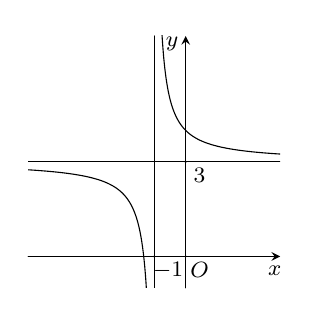
\begin{tikzpicture}[line join = round, line cap = round,>=stealth,font=\footnotesize,scale=0.4]
			\def \xmin{-5};
			\def \xmax{3};
			\def \ymin{-1};
			\def \ymax{7};
			\draw[->] (\xmin,0)--(\xmax,0) node[shift=(-110:0.2)] {$x$};
			\draw[->] (0,\ymin)--(0,\ymax) node[shift=(-150:0.2)] {$y$};
			\fill (0,0) circle(1pt) node[shift=(-45:0.25)]{$O$};
			\fill (-1,0) circle(1pt) node[shift=(-45:0.25)]{$-1$};
			\fill (0,3) circle(1pt) node[shift=(-45:0.25)]{$3$};
			\clip (\xmin,\ymin) rectangle (\xmax,\ymax); 
			\draw[smooth,samples=100] plot[domain=-0.9:\xmax] (\x,{(3*\x+4)/(\x+1)});
			\draw[smooth,samples=100] plot[domain=\xmin:-1.1] (\x,{(3*\x+4)/(\x+1)});
			\draw (\xmin,3) -- (\xmax,3);
			\draw (-1,\ymin) -- (-1,\ymax);
		\end{tikzpicture}
	}
	\loigiai{
		Quan sát đồ thị, ta thấy đây là đồ thị hàm bậc nhất trên bậc nhất với tiệm cận đứng $x=-1$ nên $y=\dfrac{3x+4}{x+1}$ là hàm số cần tìm.
	}
\end{ex}

\begin{ex}%[Đề thi thử THPT 2026 - SGD Thái Nguyên - Lần 1, Đoàn Hùng]%[2H2N2-3]
	Trong không gian với hệ tọa độ $Oxyz$, cho các véc-tơ $\overrightarrow{a} = (2;-1;-3)$, $\overrightarrow{b} = (1;-3;-2)$. Tọa độ của véc-tơ $\overrightarrow{c} = -\overrightarrow{a} + 3\overrightarrow{b}$ là
	\choice
	{$(1;8;-3)$}
	{\True $(1;-8;-3)$}
	{$(1;8;3)$}
	{$(5;-8;-3)$}
	\loigiai{
		Ta có $\heva{-\overrightarrow{a} &= (-2;1;3)\\ 3\overrightarrow{b} &= (3;-9;-6)}\Rightarrow \overrightarrow{c} = -\overrightarrow{a} + 3\overrightarrow{b} = (-2+3; 1-9; 3-6) = (1;-8;-3)$.
	}
\end{ex}

\begin{ex}%[Đề thi thử THPT 2026 - SGD Thái Nguyên - Lần 1, Đoàn Hùng]%[2H2N2-2]
	Trong không gian với hệ tọa độ $Oxyz$, hình chiếu vuông góc của điểm $M(3;2;-1)$ trên mặt phẳng $(Oxz)$ có tọa độ là
	\choice
	{$(0;2;-1)$}
	{$(3;2;0)$}
	{$(0;2;0)$}
	{\True $(3;0;-1)$}
	\loigiai{
		Hình chiếu của $M(3;2;-1)$ lên mặt phẳng $(Oxz)$ là điểm $H(3;0;-1)$.
	}
\end{ex}

\begin{ex}%[Đề thi thử THPT 2026 - SGD Thái Nguyên - Lần 1, Đoàn Hùng]%[2D1N1-2]
	\immini
	{
		Cho hàm số đa thức bậc ba $y=f(x)$ có đồ thị như hình vẽ. Hàm số đã cho nghịch biến trên khoảng nào dưới đây?
		\choice
		{$(-1; +\infty)$}
		{\True $(-\infty; -1)$}
		{$(-1; 1)$}
		{$(-\infty; 1)$}
	}
	{
		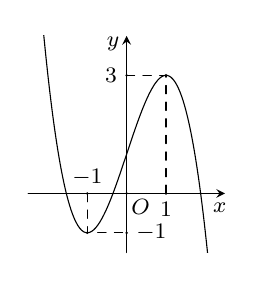
\begin{tikzpicture}[line join = round, line cap = round,>=stealth,font=\footnotesize,scale=0.5]
			\def \xmin{-2.5};
			\def \xmax{2.5};
			\def \ymin{-1.5};
			\def \ymax{4};
			\draw[->] (\xmin,0)--(\xmax,0) node[shift=(-110:0.2)] {$x$};
			\draw[->] (0,\ymin)--(0,\ymax) node[shift=(-150:0.2)] {$y$};
			\fill (0,0) circle(1pt) node[shift=(-45:0.25)]{$O$};
			\fill (-1,0) circle(1pt) node[shift=(90:0.2)]{$-1$};
			\fill (1,0) circle(1pt) node[shift=(-90:0.2)]{$1$};
			\fill (0,-1) circle(1pt) node[right]{$-1$};
			\fill (0,3) circle(1pt) node[left]{$3$};
			\fill (-1,-1) circle(1pt) (1,3) circle(1pt);
			\draw[dashed] (-1,0)|-(0,-1) (1,0)|-(0,3);
			\clip (\xmin,\ymin) rectangle (\xmax,\ymax); 
			\draw[smooth,samples=100] plot[domain=\xmin:\xmax] (\x,{-(\x)^3+3*\x+1});
		\end{tikzpicture}
	}
	\loigiai{
		Dựa vào đồ thị hàm số ta thấy hàm số đã cho nghịch biến trên các khoảng $(-\infty;-1)$ và $(1;+\infty)$.
	}
\end{ex}

\begin{ex}%[Đề thi thử THPT 2026 - SGD Thái Nguyên - Lần 1, Đoàn Hùng]%[1H4N3-2]
	\immini
	{
		Cho hình hộp $ABCD.EFGH$ (tham khảo hình vẽ). Đường thẳng $AD$ song song với mặt phẳng nào sau đây?
		\choice
		{$(ABFE)$}
		{$(ACGE)$}
		{\True $(BCGF)$}
		{$(CDHG)$}
	}
	{
		\begin{tikzpicture}[line join = round, line cap = round,>=stealth,font=\footnotesize,scale=0.5]
			\def \h{3};
			\path 
			(0,0) coordinate (A)
			(-1,-1) coordinate (B)
			(3,0) coordinate (D)
			($(B)+(D)-(A)$) coordinate (C)
			($(A)+(0,\h)$) coordinate (E)
			($(B)+(0,\h)$) coordinate (F)
			($(C)+(0,\h)$) coordinate (G)
			($(D)+(0,\h)$) coordinate (H);
			\draw[dashed] (A) -- (B) (A) -- (D) (A) -- (E);
			\draw (E) -- (F) -- (G) -- (H) -- (E) (B) -- (F) (C) -- (G) (D) -- (H) (B) -- (C) -- (D);
			\foreach \x/\g in {A/180,B/180,C/0,D/0,E/180,F/180,G/0,H/0} \fill (\x) circle (1pt)+(\g:3mm) node{$\x$};
		\end{tikzpicture}
		
	}
	\loigiai{
		Trong hình hộp $ABCD.EFGH$, ta có $AD \parallel BC$. 
		Mà $BC \subset (BCGF)$ nên $AD \parallel (BCGF)$.
	}
\end{ex}

\begin{ex}%[Đề thi thử THPT 2026 - SGD Thái Nguyên - Lần 1, Đoàn Hùng]%[1H8N7-3]
	Cho hình chóp $S.ABCD$ có $SA$ vuông góc với mặt phẳng $(ABCD)$, tứ giác $ABCD$ là hình vuông, $SA=6$ và $AB=2$. Thể tích của khối chóp $S.ABCD$ bằng
	\choice
	{\True $8$}
	{$12$}
	{$6$}
	{$24$}
	\loigiai{
		Vì $SA\perp (ABCD)$ nên $V=\dfrac{1}{3}SA\cdot S_{ABCD}=\dfrac{1}{3}SA\cdot AB^2=\dfrac{1}{3}\cdot 6\cdot 2^2=8$.
	}
\end{ex}

\begin{ex}%[Đề thi thử THPT 2026 - SGD Thái Nguyên - Lần 1, Đoàn Hùng]%[2D1N2-2]
	Cho hàm số $f(x)$ có bảng biến thiên như sau:
	\begin{center}
		
\begin{tikzpicture}
			\tkzTabInit[nocadre=false,lgt=1.2,espcl=2.5,deltacl=0.6]
			{$x$ /0.6, $f’(x)$ /0.6, $f(x)$ /2}
			{$-\infty$,$2$,$4$,$+\infty$}
			\tkzTabLine{ ,+,z,-,z,+, }
			\tkzTabVar{-/$-\infty$,+/$3$,-/$1$,+/$+\infty$}
		\end{tikzpicture}
	\end{center}
	Điểm cực đại của hàm số đã cho là
	\choice
	{\True $x=2$}
	{$x=3$}
	{$x=4$}
	{$x=1$}
	\loigiai{
		Dựa vào bảng biến thiên, hàm số đạt cực đại tại điểm $x=2$.
	}
\end{ex}

\begin{ex}%[Đề thi thử THPT 2026 - SGD Thái Nguyên - Lần 1, Đoàn Hùng]%[2D3H2-2]
	Thống kê chiều cao (đơn vị: cm) của các học sinh trong một lớp học ta có bảng số liệu sau:
	\begin{center}
		\begin{tabular}{|c|c|c|c|c|c|c|}
			\hline
			Chiều cao & $[150;155)$ & $[155;160)$ & $[160;165)$ & $[165;170)$ & $[170;175)$ & $[175;180)$ \\ \hline
			Số học sinh & $1$ & $4$ & $10$ &$9$ & $4$ & $2$ \\ \hline
		\end{tabular}
	\end{center}
	Độ lệch chuẩn (làm tròn đến hàng phần trăm) của mẫu số liệu ghép nhóm trên bằng bao nhiêu?
	\choice
	{$5{,}97$}
	{$34{,}47$}
	{$35{,}66$}
	{\True $5{,}87$}
	\loigiai{
		Ta có bảng số liệu kèm giá trị đại diện như sau:
		\begin{center}
			\begin{tabular}{|c|c|c|c|c|c|c|c|}
				\hline
				Chiều cao & $[150;155)$ & $[155;160)$ & $[160;165)$ & $[165;170)$ & $[170;175)$ & $[175;180)$& \\ \hline
				Giá trị đại diện &$152{,}5$ & $157{,}5$ & $162{,}5$ & $167{,}5$ & $172{,}5$ & $177{,}5$ &\\ 
				\hline
				Số học sinh & $1$ & $4$ & $10$ & $9$ & $4$ & $2$ &$n=30$\\ 
				\hline
			\end{tabular}
		\end{center}
		Số trung bình: $\bar{x} = \dfrac{1\cdot 152{,}5 + 4\cdot 157{,}5 + 10\cdot 162{,}5 + 9\cdot 167{,}5 + 4\cdot 172{,}5 + 2\cdot 177{,}5}{30} = 165{,}1(6)$.\\
		Độ lệch chuẩn
		\begin{align*}
			\sqrt{\dfrac{(152{,}5-\overline{x})^2+4\cdot (157{,}5-\overline{x})^2+10\cdot (162{,}5-\overline{x})^2+\ldots+2\cdot \left(177{,}5-\overline{x}\right)^2}{30}}\approx 5{,}87.
		\end{align*}
	}
\end{ex}

\begin{ex}%[Đề thi thử THPT 2026 - SGD Thái Nguyên - Lần 1, Đoàn Hùng]%[2D4N1-4]
	Các nguyên hàm của hàm số $f(x) = 7^x + \dfrac{x}{3}$ là
	\choice
	{$7^x + \dfrac{2x^2}{3} + C$}
	{$\dfrac{7^x}{\ln 7} + \dfrac{x^2}{3} + C$}
	{$7^x \ln 7 + \dfrac{x^2}{6} + C$}
	{\True $\dfrac{7^x}{\ln 7} + \dfrac{x^2}{6} + C$}
	\loigiai{
		Ta có $\displaystyle\int \left( 7^x + \dfrac{x}{3} \right) \mathrm{\,d}x = \displaystyle\int 7^x \mathrm{\,d}x + \dfrac{1}{3} \displaystyle\int x \mathrm{\,d}x = \dfrac{7^x}{\ln 7} + \dfrac{1}{3} \cdot \dfrac{x^2}{2} + C = \dfrac{7^x}{\ln 7} + \dfrac{x^2}{6} + C$.
	}
\end{ex}

\begin{ex}%[Đề thi thử THPT 2026 - SGD Thái Nguyên - Lần 1, Đoàn Hùng]%[1D2N3-2]
	Cho cấp số nhân $(u_n)$ có $u_1 = 2$ và $u_4 = 54$. Công bội của cấp số nhân đã cho bằng
	\choice
	{\True $3$}
	{$-4$}
	{$4$}
	{$2$}
	\loigiai{
		Ta có $u_4=u_1\cdot q^3\Rightarrow q^3=\dfrac{u_4}{u_1}=\dfrac{54}{2}=27\Rightarrow q=3$.
	}
\end{ex}
\Closesolutionfile{ans}


\cauds
\Opensolutionfile{ans}[ans/ans-26-2--SoGDThaiNguyen-L1-DS]
\begin{ex}%[Đề thi thử THPT 2026 - SGD Thái Nguyên - Lần 1, Đoàn Hùng]%[1D1V5-6]
	Khi kéo ra khỏi vị trí cân bằng ở điểm $O$ và buông tay, lực đàn hồi của lò xo khiến vật $A$ gắn ở đầu của lò xo dao động quanh $O$ như hình vẽ sau:
	\begin{center}
		\begin{tikzpicture}[line join = round, line cap = round,>=stealth,font=\footnotesize,scale=1]
			% Vẽ mặt sàn và tường
			\fill[pattern=north east lines] (-0.2,0) rectangle (6,-0.2); % Mặt sàn
			
			\fill[pattern=north west lines] (-0.2,0) rectangle (0,1.5); % Tường
			\draw[thick] (0,0) -- (0,1.5);
			\path 
			(2.5,0.4) coordinate (M)
			(3.5,0.4) coordinate (O)
			(6,0.4) coordinate (x)
			(0,0.4) coordinate (N)
			;
			\draw[->] (N) -- (x) node[above] {$x$};
			\fill (O) circle (1pt) node[below] {$O$};
			% Vẽ vật nặng A
			% Giả sử vật A là một hình vuông, tâm vật tại điểm M
			
			\draw[thick, fill=white] (2,0) rectangle (3,0.8);
			\node at (2.5,1) {$A$};
			\fill (M) circle (1.5pt);
			
			% Vẽ lò xo (Spring)
			\draw[decoration={aspect=0.3, segment length=1.5mm, amplitude=2mm, coil}, decorate] 
			(0,0.4) -- (2,0.4);
			\draw (0,0) -- (6,0);
		\end{tikzpicture}
	\end{center}
	Tọa độ $s$ (centimét) của $A$ trên trục $Ox$ vào thời điểm $t$ (giây) sau khi buông tay được xác định bởi công thức $s = 8\sin\left(10t - \dfrac{\pi}{2}\right)$.
	\choiceTF
	{\True Tập xác định của hàm số $s = 8\sin\left(10t - \dfrac{\pi}{2}\right)$ là $\mathbb{R}$}
	{Giá trị lớn nhất của hàm số $s = 8\sin\left(10t - \dfrac{\pi}{2}\right)$ bằng $1$}
	{Thời điểm đầu tiên tọa độ của vật $A$ trên trục bằng $4$ là $t = \dfrac{2\pi}{15}$ (giây)}
	{\True Trong $2$ giây đầu tiên vật đi qua vị trí cân bằng $6$ lần}
	\loigiai{
		\begin{itemchoice}
			\itemch Hàm số lượng giác $y = \sin(at+b)$ luôn có tập xác định là $\mathbb{R}$.
			\itemch Với mọi $t>0$, ta có $-1 \le \sin\left(10t - \dfrac{\pi}{2}\right) \le 1$ nên $-8 \le s \le 8$. \\
			Suy ra giá trị lớn nhất của hàm số $s = 8\sin\left(10t - \dfrac{\pi}{2}\right)$ bằng $8$.
			\itemch Vật ở vị trí $s=4$, ta có 
			\begin{eqnarray*}
				8\sin\left(10t - \dfrac{\pi}{2}\right) = 4 &\Leftrightarrow& \sin\left(10t - \dfrac{\pi}{2}\right) = \dfrac{1}{2}\\
				&\Leftrightarrow& \hoac{& 10t-\dfrac{\pi}{2}=\dfrac{\pi}{6}+k2\pi \\ & 10t-\dfrac{\pi}{2}=\dfrac{5\pi}{6}+k2\pi}\\
				&\Leftrightarrow& \hoac{& t=\dfrac{\pi}{15}+\dfrac{k2\pi}{5} \\ & t=\dfrac{2\pi}{15}+\dfrac{k2\pi}{5}}, k \in \mathbb{Z}.
			\end{eqnarray*}
			Vì $t > 0$ nên thời điểm đầu tiên là $t_0 = \dfrac{\pi}{15}$ giây.
			\itemch Vị trí cân bằng là $s=0$, ta có 
			$$\sin\left(10t - \dfrac{\pi}{2}\right) = 0 \Leftrightarrow 10t - \dfrac{\pi}{2} = k\pi \Leftrightarrow t = \dfrac{\pi}{20} + \dfrac{k\pi}{10}, k \in \mathbb{Z}.$$
			Với $0 \le t \le 2$, ta có $0 \le \dfrac{\pi}{20} + \dfrac{k\pi}{10} \le 2 \Rightarrow -0,5 \le k \le 5,86$.\\
			Vì $k\in \mathbb{Z}$ nên $k \in \{0; 1; 2; 3; 4; 5\}$.\\
			Vậy trong $2$ giây đầu tiên, vật đi qua vị trí cân bằng $6$ lần.
		\end{itemchoice}
	}
\end{ex}

\begin{ex}%[Đề thi thử THPT 2026 - SGD Thái Nguyên - Lần 1, Đoàn Hùng]%[2D1V4-1]
	Cho hàm số $y = \dfrac{x^2 - x - 1}{x - 2}$.
	\choiceTF
	{Hàm số nghịch biến trên khoảng $(1;3)$}
	{\True Giả sử $y_1$, $y_2$ là hai giá trị cực trị của hàm số đã cho. Khi đó, giá trị $y_1 \cdot y_2 = 5$}
	{\True Đường tiệm cận xiên của đồ thị hàm số là $y = x + 1$}
	{\True Gọi $A$, $B$ lần lượt là điểm cực đại, điểm cực tiểu của đồ thị hàm số đã cho và $C(-1;3)$. Khi đó, diện tích tam giác $ABC$ bằng $6$ (đvdt)}
	\loigiai{
		Hàm số đã cho có tập xác định $\mathscr{D}=\mathbb{R}\setminus \{2\}$.\\
		Ta có $y' = \dfrac{x^2 - 4x + 3}{(x-2)^2}$.\\
		Phương trình $ y'= 0 \Leftrightarrow \hoac{&x=1\\&x=3.}$ \\
		Bảng biến thiên của hàm số như sau:
		\begin{center}
			
\begin{tikzpicture}
				\tkzTabInit[nocadre=false,lgt=1.2,espcl=2.5,deltacl=0.6]
				{$x$ /0.6, $f’(x)$ /0.6, $f(x)$ /2}
				{$-\infty$,$1$,$2$,$3$,$+\infty$}
				\tkzTabLine{ ,+,$0$,-,d,-,$0$,+, }
				\tkzTabVar{-/$-\infty$,+/$1$,-D+/$-\infty$/$+\infty$,-/$5$,+/$+\infty$}
			\end{tikzpicture}
		\end{center}
		\begin{itemchoice}
			\itemch Hàm số không xác định tại $x=2 \in (1;3)$ nên không thể nghịch biến trên toàn khoảng $(1;3)$.
			\itemch Từ bảng biến tiên, suy ra hàm số đã cho có giá trị cực đại $y_1=1$ và giá trị cực tiểu $y_2=5$.\\
			Suy ra $y_1\cdot y_2=1\cdot 5=5$.
			\itemch Ta có $y = \dfrac{x^2 - x - 1}{x - 2} = x + 1 + \dfrac{1}{x-2}$.\\
			Do đó $\lim \limits_{x \to +\infty} \left[y-\left(x+1\right)\right]=\lim \limits_{x \to +\infty}\dfrac{1}{x-2}=0$ và $\lim \limits_{x \to -\infty} \left[y-\left(x+1\right)\right]=\lim \limits_{x \to -\infty}\dfrac{1}{x-2}=0$.\\
			Suy ra $y=x+1$ là tiệm cận xiên của đồ thị hàm số.
			\itemch Đồ thị của hàm số đã cho có điểm cực đại $A(1;1)$ và điểm cực tiểu $B(3;5)$ và $AB=2\sqrt{5}$.\\
			Đường thẳng $AB$ có phương trình $\dfrac{x-1}{3-1}=\dfrac{y-1}{5-1} \Leftrightarrow 2x-y-1=0$.\\
			Do đó $\mathrm{d}(C,AB)=\dfrac{|2\cdot (-1)-3-1|}{\sqrt{2^2+(-1)^2}}=\dfrac{6\sqrt{5}}{5}$.\\
			Suy ra $S_{\triangle ABC}=\dfrac{1}{2}\mathrm{d}(C,AB)\cdot AB=\dfrac{1}{2}\cdot \dfrac{6\sqrt{5}}{5}\cdot 2\sqrt{5}=6$.
		\end{itemchoice}
	}
\end{ex}

\begin{ex}%[Đề thi thử THPT 2026 - SGD Thái Nguyên - Lần 1, Đoàn Hùng]%[2H2C2-4]
	Trong không gian với hệ tọa độ $Oxyz$, cho hình thang $ABCD$ vuông tại $A$ và $B$. Biết $A(1;2;1)$, $B(2;0;-1)$, $C(6;1;0)$ và diện tích hình thang $ABCD$ bằng $21\sqrt{2}$.
	\choiceTF
	{\True $\overrightarrow{BC} \cdot \overrightarrow{CA} = -18$}
	{\True $\cos\left(\overrightarrow{BC}, \overrightarrow{CA}\right) = -\dfrac{\sqrt{6}}{3}$}
	{\True Tọa độ điểm $D$ là $(a;b;c)$. Khi đó $a+b+c = 26$}
	{Gọi điểm $M(x_M; y_M; z_M)$ nằm trên mặt phẳng $(Oyz)$ thỏa mãn $MA^2 + 2MB^2 + 5MC^2$ đạt giá trị nhỏ nhất. Khi đó $y_M > 1$}
	\loigiai{
		\begin{center}
			\begin{tikzpicture}[line join = round, line cap = round,>=stealth,font=\footnotesize,scale=1]
				\path 
				(0,0) coordinate (B)
				($(B)+(2,0)$) coordinate (C)
				(0,-2) coordinate (A)
				($(A)+(5,0)$) coordinate (D)
				;
				\draw (A) -- (B) -- (C) -- (D) -- (A);
				\foreach \x/\g in {A/-90,B/90,C/90,D/-90} \fill (\x) circle (1pt)+(\g:3mm) node{$\x$};
				\draw 
				pic [draw, angle radius = 2.2mm]{right angle = A--B--C}
				pic [draw, angle radius = 2.2mm]{right angle = B--A--D}
				;
			\end{tikzpicture}
		\end{center}
		\begin{itemchoice}
			\itemch Ta có $\overrightarrow{BC} = (4;1;1)$, $\overrightarrow{CA} = (-5;1;1)$.\\
			Suy ra $\overrightarrow{BC}\cdot \overrightarrow{CA}=4\cdot (-5)+1\cdot 1+1\cdot 1=-18$.
			\itemch Ta có 
			$$\cos\left(\overrightarrow{BC}, \overrightarrow{CA}\right) = \dfrac{\overrightarrow{BC} \cdot \overrightarrow{CA}}{\left|\overrightarrow{BC}\right| \cdot \left|\overrightarrow{CA}\right|} = \dfrac{-18}{\sqrt{18} \cdot \sqrt{27}} = -\dfrac{18}{3\sqrt{2} \cdot 3\sqrt{3}} = -\dfrac{2}{\sqrt{6}} = -\dfrac{\sqrt{6}}{3}.$$
			\itemch Vì $ABCD$ vuông tại $A$, $B$ nên $AD \parallel BC$. 	\\
			Ta có $BC=\sqrt{4^2+1^2+1^2}=3\sqrt{2}$, $AB=\sqrt{1^2+(-2)^2+(-2)^2}=3$.\\
			Do đó $S_{ABCD}=\dfrac{AB(AD+BC)}{2}=\dfrac{3\left(AD+3\sqrt{2}\right)}{2}$.\\
			Theo giả thiết, ta có $S_{ABCD}=21\sqrt{2}$, suy ra 
			$$\dfrac{3\left(AD+3\sqrt{2}\right)}{2}=21\sqrt{2}\Rightarrow AD=11\sqrt{2}\Rightarrow \overrightarrow{AD}=\dfrac{11}{3}\overrightarrow{BC}.$$
			Suy ra $\heva{& a-1=\dfrac{11}{3}\cdot 4 \\ & b-2=\dfrac{11}{3}\\& c-1=\dfrac{11}{3}} \Rightarrow \heva{&a=\dfrac{47}{3}\\&b=\dfrac{17}{3}\\&c=\dfrac{14}{3}.}$\\
			Vậy $a+b+c=\dfrac{47+17+14}{3}=26$.
			\itemch Gọi $G$ là điểm thoả mãn $\overrightarrow{GA}+2\overrightarrow{GB}+5\overrightarrow{GC}=\overrightarrow{0}$. Khi đó, ta có
			$$\overrightarrow{OG}=\dfrac{1}{1+2+5}\left(\overrightarrow{OA}+2\overrightarrow{OB}+5\overrightarrow{OC}\right)\Rightarrow G\left(\dfrac{35}{8};\dfrac{7}{8};-\dfrac{1}{8}\right).$$\
			Mặt khác, ta có 
			\begin{eqnarray*}
				MA^2+2MB^2+5MC^2&=&\left(\overrightarrow{GA}-\overrightarrow{GM}\right)^2+2\left(\overrightarrow{GB}-\overrightarrow{GM}\right)^2+5\left(\overrightarrow{GC}-\overrightarrow{GM}\right)^2\\
				&=&GA^2+2GB^2+5GC^2+8GM^2.
			\end{eqnarray*}
			Vì $G$ là điểm cố định nên $GA^2+2GB^2+5GC^2$ không đổi.\\
			Suy ra $MA^2+2MB^2+5MC^2$ đạt giá trị nhỏ nhất khi và chỉ khi $MG$ đạt giá trị nhỏ nhất hay $M$ là hình chiếu vuông góc của điểm $G$ lên mặt phẳng $(Oyz)$.\\
			Suy ra $ M\left(0;\dfrac{7}{8};-\dfrac{1}{8}\right)$.\\
			Vậy $y_M=\dfrac{7}{8}<1$.
		\end{itemchoice}
	}
\end{ex}

\begin{ex}%[Đề thi thử THPT 2026 - SGD Thái Nguyên - Lần 1, Đoàn Hùng]%[2D1V3-6]
	Tại một lễ hội dân gian, tốc độ thay đổi lượng khách tham dự sau $t$ giờ kể từ khi bắt đầu khai mạc được biểu diễn bằng hàm số $B'(t) = 20t^3 - 300t^2 + 1000t$ (đơn vị: khách/giờ), với $0 \le t \le 15$. Sau một giờ, $500$ người đã có mặt tại lễ hội.
	\choiceTF
	{\True Tốc độ thay đổi lượng khách tham dự lễ hội này tại thời điểm $1$ giờ kể từ khi bắt đầu khai mạc bằng $720$ khách/giờ}
	{Công thức của hàm số $B(t)$ biểu diễn số lượng khách tham dự lễ hội, với $0 \le t \le 15$ là $B(t) = 5t^4 - 100t^3 + 500t^2 + C$ (với $C$ là một hằng số tùy ý)}
	{\True Sau $3$ giờ kể từ khi bắt đầu khai mạc, lễ hội có $2300$ khách tham dự}
	{\True Sau $15$ giờ kể từ khi bắt đầu khai mạc thì số lượng khách tham dự lễ hội là đông nhất}
	\loigiai{
		\begin{itemchoice}
			\itemch Thay $t=1$ vào $B'(t)$, ta được $B'(1) = 20(1)^3 - 300(1)^2 + 1000(1) = 720$.
			\itemch Ta có $\displaystyle\int B'(t) \mathrm{\,d}t = 5t^4 - 100t^3 + 500t^2 + C$, $C\in \mathbb{R}$.\\
			Hàm số $B(t)$ là một nguyên hàm của $B'(t)$ thỏa mãn $B(1) = 500$ nên $C = 95$.\\
			Suy ra $B(t)=5t^4 - 100t^3 + 500t^2 + 95$.\\ 
			Hằng số $C=95$ xác định từ điều kiện thực tế nên không thể là một hằng số tùy ý.
			\itemch Ta có $B(t)=5t^4 - 100t^3 + 500t^2 + 95$, với $t \ge 0$.\\ \\
			Lượng khách tham gia lễ hội sau $3$ giờ là $B(3) = 2300$.
			\itemch Ta có $B'(t)=0\Leftrightarrow 20t^3-300t^2+1000t=0\Leftrightarrow \hoac{& t=0 \\ & t=5\\& t=10.}$\\
			Lại có $B(0)=95$; $B(5)=3\,220$; $B(10)=95$; $B(15)=28\,220$.\\
			Vậy sau $15$ giờ kể từ khi bắt đầu khai mạc, số lượng khác tham dự lễ hội là đông nhất với $28\,220$ khách.
		\end{itemchoice}
	}
\end{ex}

\Closesolutionfile{ans}

\caukq
\Opensolutionfile{ans}[ans/ans-26-2--SoGDThaiNguyen-L1-KQ]
\begin{ex}%[Đề thi thử THPT 2026 - SGD Thái Nguyên - Lần 1, Đoàn Hùng]%[2D4H1-6]
	Đối với ngành nuôi trồng thủy sản, việc kiểm soát lượng thuốc tồn dư trong nước là một nhiệm vụ quan trọng nhằm đáp ứng các tiêu chuẩn an toàn về môi trường. Khi nghiên cứu một loại thuốc trị bệnh trong nuôi trồng thủy sản, người ta sử dụng thuốc đó một lần và theo dõi nồng độ thuốc tồn dư trong nước kể từ lúc sử dụng thuốc. Kết quả cho thấy nồng độ thuốc $y(t)$ (đơn vị: mg/lít) tồn dư trong nước tại thời điểm $t$ ngày kể từ lúc sử dụng thuốc, thỏa mãn $y(t) = \mathrm{e}^{g(t)}$ và $y'(t) = k \cdot y(t)$ với $t \ge 0$, trong đó $k$ là hằng số khác không. Đo nồng độ thuốc tồn dư trong nước tại các thời điểm $t=5$ ngày, $t=10$ ngày nhận được kết quả lần lượt là $3$ mg/lít, $1$ mg/lít. Nồng độ thuốc tồn dư trong nước tại thời điểm $15$ ngày bằng bao nhiêu mg/lít (kết quả làm tròn đến hàng phần trăm)?
	\par \shortans{$0{,}33$}
	\loigiai
	{
		Ta có $y'(t)=\mathrm{e}^{g(t)}\cdot g'(t)=k\cdot \mathrm{e}^{g(t)}\Rightarrow g'(t)=k$ là hằng số, suy ra $g(t)=kt+b\Rightarrow y(t)=\mathrm{e}^{kt+b}$.\\
		Đo nồng độ thuốc tồn dư trong nước tại các thời điểm $t=5$ ngày, $t=10$ ngày nhận được kết quả lần lượt là $3$ mg/lít, $1$ mg/lít nên ta có hệ phương trình
		\begin{align*}
			\heva{& \mathrm{e}^{5k+b}=3 \\ & \mathrm{e}^{10k+b}=1} \Leftrightarrow \heva{& \mathrm{e}^{5k}\cdot \mathrm{e}^{b}=3 \\ & \mathrm{e}^{5k}=\dfrac{1}{3}} \Leftrightarrow \heva{& \mathrm{e}^{5k}=\dfrac{1}{3} \\ & \mathrm{e}^{b}=9.}
		\end{align*}
		Sau $15$ ngày thì nồng độ thuốc tồn dư trong nước là $$\mathrm{e}^{15k+b}=\mathrm{e}^{15k}\cdot \mathrm{e}^{b}=\left(\mathrm{e}^{5k}\right)^{3}\cdot \mathrm{e}^{b}=\left(\dfrac{1}{3}\right)^3\cdot 9=\dfrac{1}{3}\approx 0{,}33.$$
	}
\end{ex}

\begin{ex}%[Đề thi thử THPT 2026 - SGD Thái Nguyên - Lần 1, Đoàn Hùng]%[2H2V2-6]
	Cho hình hộp chữ nhật $ABCD.EFGH$ với $AB=6$, $AD=8$ và $DH=10$. Gọi điểm $M$ là trung điểm của đoạn thẳng $AF$ và điểm $I$ thuộc mặt phẳng $(ABCD)$. Khi $IM+IG$ nhỏ nhất thì điểm $I$ cách hai đường thẳng $BA$ và $BC$ tương ứng bằng $p$ và $q$. Giá trị của biểu thức $Q=3p+q$ bằng bao nhiêu?
	\par \shortans{$10$}
	\loigiai{
		\begin{center}
			\begin{tikzpicture}[line join = round, line cap = round,>=stealth,font=\footnotesize,scale=1]
				\def \h{4}
				\path 
				(0,0) coordinate (A)
				($(A)+(4,0)$) coordinate (D)
				($(A)+(1.7,-0.6)$) coordinate (I)
				($(A)+(-1.5,-1.5)$) coordinate (B)
				($(B)+(D)-(A)$) coordinate (C)
				($(A)+(0,\h)$) coordinate (E)
				($(B)+(0,\h)$) coordinate (F)
				($(C)+(0,\h)$) coordinate (G)
				($(D)+(0,\h)$) coordinate (H)
				($(A)!0.5!(F)$) coordinate (M)
				($(A)!0.5!(B)$) coordinate (N)
				($(M)!2!(N)$) coordinate (M')
				($(A)!1.5!(B)$) coordinate (x)
				($(A)!1.3!(D)$) coordinate (y)
				($(A)!1.2!(E)$) coordinate (z)
				(intersection of C--N and M'--G) coordinate (I_1)
				($(A)+(1.7,-0.6)$) coordinate (I)
				(intersection of I--M' and B--C) coordinate (P)
				(intersection of G--M' and B--C) coordinate (Q)
				(intersection of M--M' and B--C) coordinate (R)
				;
				\draw (E) -- (F) -- (G) -- (H) -- (E)  (F) -- (B) (G) -- (C) (H) -- (D) -- (C) -- (B) (P) -- (M') -- (Q) (M') -- (R);
				\draw[dashed] (E) -- (A) -- (B) (A) -- (D) (A) -- (F) (M) -- (R) -- (Q) -- (G) -- (I) -- (M) (I) -- (P);
				\draw[->] (B) -- (x) node[below] {$x$};
				\draw[->] (D) -- (y) node[above] {$y$};
				\draw[->] (E) -- (z) node[right] {$z$};
				\foreach \x/\g in {A/180,B/180,C/0,D/50,E/180,F/180,G/0,H/0,M/30,M'/-90,I/-30} \fill[black](\x) circle (1pt)+(\g:4mm) node{$\x$};
				\fill (I_1) circle (1pt);
			\end{tikzpicture}
		\end{center}
		Gán các trục toạ độ như hình vẽ, với $A\equiv O(0,0,0)$.\\
		Khi đó $A(0;0;0)$, $B(6;0;0)$, $D(0;8;0)$, $E(0;0;10)$, $F(6;0;10)$, $C(6;8;0)$, $G(6;8;10)$.\\
		Vì $M$ là trung điểm của $AF$ nên $M(3;0;5)$.\\
		Gọi $M'$ là điểm đối xứng của $M$ qua $(ABCD)\Rightarrow M'(3;0;-5)$.\\
		Ta có $IM+IG=IM'+IG\geq M'G$.\\
		Dấu \lq\lq =\rq\rq \text{} xảy ra khi và chỉ khi $M'$, $I$, $G$ thẳng hàng.\\
		Vì $I\in (xOy)$ nên $I(x;y;0)\Rightarrow \overrightarrow{M'G}=(3;8;15)$, $\overrightarrow{M'I}=(x-3;y;5)$.\\
		Vì $M'$, $I$, $G$ thẳng hàng nên $\dfrac{x-3}{3}=\dfrac{y}{8}=\dfrac{5}{15}=\dfrac{1}{3}\Rightarrow \heva{& x=4 \\ & y=\dfrac{8}{3}}\Rightarrow I\left(4;\dfrac{8}{3};0\right)$.\\
		Khoảng cách từ $I$ đến $AB$ là $y=\dfrac{8}{3}$, khoảng cách từ $I$ đến $BC$ là $6-x=2$.\\
		Do đó $p=\dfrac{8}{3}$, $q=2\Rightarrow 3p+q=8+2=10$.
	}
\end{ex}

\begin{ex}%[Đề thi thử THPT 2026 - SGD Thái Nguyên - Lần 1, Đoàn Hùng]%[1H8H6-2]
	Người ta dự định dùng hai loại nguyên liệu để chiết xuất ít nhất $190$ kg chất $A$ và $13$ kg chất $B$. Từ mỗi tấn nguyên liệu loại $I$ giá $5$ triệu đồng, có thể chiết xuất được $25$ kg chất $A$ và $0{,}5$ kg chất $B$. Từ mỗi tấn nguyên liệu loại $II$ giá $4$ triệu đồng, có thể chiết xuất được $10$ kg chất $A$ và $2{,}5$ kg chất $B$. Biết rằng cơ sở cung cấp nguyên liệu chỉ có thể cung cấp không quá $12$ tấn nguyên liệu loại $I$ và không quá $8$ tấn nguyên liệu loại $II$. Hỏi chi phí để mua nguyên liệu ít nhất bằng bao nhiêu triệu đồng?
	\par \shortans{$46$}
	\loigiai
	{
		\immini
		{
			Gọi khối lượng nguyên liệu loại $I$ là $x$ (tấn).\\
			Gọi khối lượng nguyên liệu loại $II$ là $y$ (tấn).\\
			$x$ tấn nguyên liệu loại $I$ sản xuất được $25x$ kg chất $A$ và $0{,}5x$ kg chất $B$.\\
			$y$ tấn nguyên liệu loại $II$ sản xuất được $10y$ kg chất $A$ và $2{,}5y$ kg chất $B$.\\
			Theo đề bài ta có hệ bất phương trình
			\begin{align*}
				\heva{& 0\leq x\leq 12,\,0\leq y\leq 8 \\ & 25x+10y\geq 190\\& 0{,}5x+2{,}5y\geq 13}\Leftrightarrow \heva{& 0\leq x\leq 12,\,0\leq y\leq 8 \\ & 5x+2y\geq 38\\& x+5y\geq 26.}
			\end{align*}
			Chi phí mua nguyên liệu là $F(x;y)=5x+4y$.\\
			Miền nghiệm của hệ bất phương trình là miền trong tứ giác $ABCD$ (kể cả các cạnh của tứ giác), với $A(4.4;8)$, $B(6,4)$, $C(12;2.8)$, $D(12;8)$.\\
			Tính giá trị của biểu thức $F$ tại các đỉnh của tứ giác này ta được \\
			$F(4.4;8)=54$; $F(6;4)=46$; $F(12;2{,}8)=71{,}2$; $F(12;8)=92$.\\
			Vậy chi phí mua nguyên liệu ít nhất là $46$ (triệu đồng).
		}
		{
			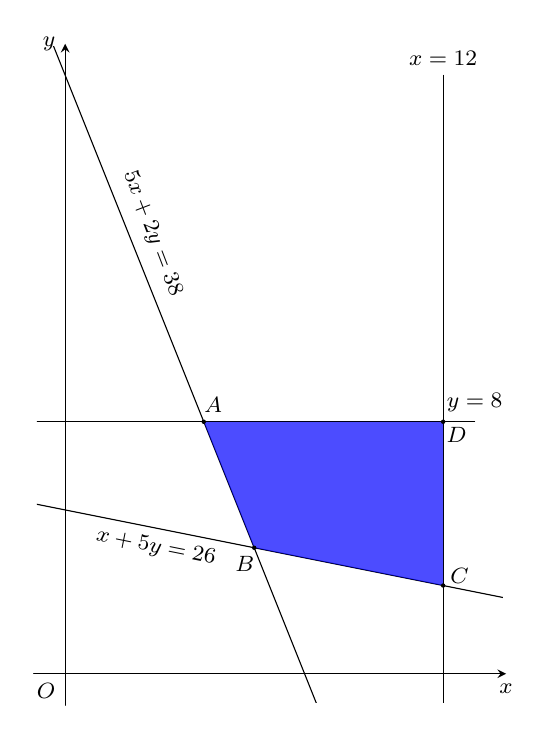
\begin{tikzpicture}[line join = round, line cap = round,>=stealth,font=\footnotesize,scale=0.4]
				\def \xmin{-1};
				\def \xmax{14};
				\def \ymin{-1};
				\def \ymax{20};
				\draw[->] (\xmin,0) -- (\xmax,0) node[below] {$x$};
				\draw[->] (0,\ymin) -- (0,0) node[below left] {$O$} -- (0,\ymax) node[left] {$y$};
				\clip (\xmin+0.1,\ymin+0.1) rectangle (\xmax-0.1,\ymax-0.1);
				\draw[smooth,samples=100] plot[domain=\xmin:\xmax] (\x,{-2.5*(\x)+19});
				\draw[smooth,samples=100] plot[domain=\xmin:\xmax] (\x,{-0.2*(\x)+5.2});
				\draw (12,\ymin) -- (12,\ymax-1) node[above] {$x=12$};
				\draw (\xmin,8) -- (\xmax-1,8) node[above] {$y=8$};
				\path 
				(4.4,8) coordinate (A)
				(6,4) coordinate (B)
				(12,2.8) coordinate (C)
				(12,8) coordinate (D)
				;
				\fill[color=blue,opacity=0.7] (A) -- (B) -- (C) -- (D) -- cycle;
				\foreach \x/\g in {A/60,B/-120,C/30,D/-45} \fill[black](\x) circle (2pt)+(\g:6mm) node{$\x$};
				
				\draw[draw=none] (0,19.5)--(A) node[midway,sloped,above]{$5x+2y=38$};
				\draw[draw=none] (0,5.2)--(B) node[midway,sloped,below]{$x+5y=26$};
			\end{tikzpicture}
		}
	}
\end{ex}

\begin{ex}%[Đề thi thử THPT 2026 - SGD Thái Nguyên - Lần 1, Đoàn Hùng]%[1H8V6-2]
	Cho tứ diện $ABCD$ có $\widehat{BAC}=30^\circ$, $\widehat{CAD}=\widehat{DAB}=60^\circ$. Gọi $\alpha = [B; AD; C]$ thì giá trị của $\cos \alpha$ bằng bao nhiêu (không làm tròn kết quả các phép tính trung gian, chỉ làm tròn kết quả cuối cùng đến hàng phần trăm)?
	\par \shortans{$0{,}82$}
	\loigiai{
		\begin{center}
			\begin{tikzpicture}[line join = round, line cap = round,>=stealth,font=\footnotesize,scale=1]
				\path
				(0,0) coordinate (B)
				(5,0) coordinate (D)
				(2.5,4) coordinate (A)
				(1,-2) coordinate (C)
				($(A)!0.3!(D)$) coordinate (H)
				($(A)!0.8!(C)$) coordinate (C')
				;
				\draw (A) -- (C) (A) -- (B) -- (C) -- (D) --cycle (H) -- (C') -- (B);
				\draw[dashed] (B) -- (D) (B) -- (H);
				\foreach \x/\g in {A/90,B/180,C/-90,D/0,H/30,C'/-60} \fill[black](\x) circle (1pt)+(\g:3mm) node{$\x$};
				\draw 
				pic [draw, angle radius = 2.5mm]{right angle = B--H--A}
				pic [draw, angle radius = 2.5mm]{right angle = C'--H--D}
				;
				
			\end{tikzpicture}
		\end{center}
		Không mất tính tổng quát ta giả sử $AC\geq AB$.\\
		Kẻ $BH\perp AD$ ($H\in AD$) và $C'H\perp AD$ ($C'\in AC$). Khi đó $\alpha = [B; AD; C]=\widehat{BHC'}.$\\
		Ta có $\triangle AHB=\triangle AHC'$ (g.c.g).\\
		Suy ra $AB=AC'=a$, $HB=HC'=AB\sin 60^\circ=\dfrac{a\sqrt{3}}{2}$.\\
		Xét $\triangle ABC'$ có
		\begin{align*}
			BC'^2=AB^2+AC'^2-2AB\cdot AC'\cdot \cos \widehat{BAC}=a^2+a^2-2a^2\cdot \dfrac{\sqrt{3}}{2}=a^2\left(2-\sqrt{3}\right).
		\end{align*}
		Xét $\triangle BHC'$ có $\cos \alpha=\cos \widehat{BHC'}=\dfrac{HB^2+HC'^2-BC'^2}{2\cdot HB\cdot HC'}=\dfrac{2\sqrt{3}-1}{3}\approx 0{,}82$.
	}
\end{ex}

\begin{ex}%[Đề thi thử THPT 2026 - SGD Thái Nguyên - Lần 1, Đoàn Hùng]%[1D9C1-3]
	Tung đồng thời hai con xúc xắc khác nhau đều cân đối và đồng chất ba lần. Bằng cách cộng số chấm xuất hiện trên hai con xúc xắc trong mỗi lần tung ta được một số ngẫu nhiên từ $2$ đến $12$. Gọi ba số này lần lượt là $a$, $b$ và $t$. Chọn ngẫu nhiên một tam giác có hai cạnh có độ dài là $a$, $b$ và góc xen giữa chúng bằng $(t-1) \cdot 15$ độ. Xác suất để tam giác này là tam giác vuông bằng bao nhiêu (kết quả làm tròn đến hàng phần trăm)?
	\par \shortans{$0{,}17$}
	\loigiai
	{
		\begin{itemize}
			\item Xác suất tổng số chấm xuất hiện trên hai con xúc xắc là $2$ bằng xác suất tổng số chấm xuất hiện trên hai con xúc xắc là $12$ và bằng $\dfrac{1}{6}\cdot \dfrac{1}{6}=\dfrac{1}{36}$.
			\item Xác suất tổng số chấm xuất hiện trên hai con xúc xắc là $3$ bằng xác suất tổng số chấm xuất hiện trên hai con xúc xắc là $11$ và bằng $2\cdot\dfrac{1}{6}\cdot \dfrac{1}{6}=\dfrac{1}{18}$ (do có $2$ bộ là $(1;2)$ và $(2;1)$).
			\item Xác suất tổng số chấm xuất hiện trên hai con xúc xắc là $4$ bằng xác suất tổng số chấm xuất hiện trên hai con xúc xắc là $10$ và bằng $3\cdot\dfrac{1}{6}\cdot \dfrac{1}{6}=\dfrac{1}{12}$ (do có $3$ bộ là $(1;3)$; $(3;1)$ và $(2;2)$).
			\item Xác suất tổng số chấm xuất hiện trên hai con xúc xắc là $5$ bằng xác suất tổng số chấm xuất hiện trên hai con xúc xắc là $9$ và bằng $4\cdot\dfrac{1}{6}\cdot \dfrac{1}{6}=\dfrac{1}{9}$ (do có $4$ bộ là $(1;4)$; $(4;1)$; $(2;3)$; $(3;2)$).
			\item Xác suất tổng số chấm xuất hiện trên hai con xúc xắc là $6$ bằng xác suất tổng số chấm xuất hiện trên hai con xúc xắc là $8$ và bằng $5\cdot\dfrac{1}{6}\cdot \dfrac{1}{6}=\dfrac{5}{36}$ (do có $5$ bộ là $(1;5)$; $(5;1)$; $(2;4)$; $(4;2)$ và $(3;3)$).
			\item Xác suất tổng số chấm xuất hiện trên hai con xúc xắc là $7$ bằng $6\cdot\dfrac{1}{6}\cdot \dfrac{1}{6}=\dfrac{1}{6}$ (do có $6$ bộ là $(1;6)$; $(6;1)$; $(2;5)$; $(5;2)$; $(3;4)$ và $(4;3)$).
		\end{itemize}
		Xét $\triangle ABC$ có $AB=a$, $AC=b$ và $\widehat{BAC}=(t-1)\cdot 15^\circ$.\\
		Gọi $A$ là biến cố $\triangle ABC$ vuông.
		\begin{itemize}
			\item Trường hợp $1$: $\triangle ABC$ vuông tại $A$. Khi đó $(t-1)\cdot 15^\circ=90^\circ\Leftrightarrow t=7$. 
			\item Trường hợp $2$: $\triangle ABC$ vuông tại $B$ hoặc $C$.\\
			Khi đó $\widehat{BAC}=(t-1)\cdot 15^\circ<90^\circ\Rightarrow t<7\Rightarrow t\in \{2;3;4;5;6\}$.\\
			Suy ra $\cos (t-1)15^\circ\in \{\cos 15^\circ;\cos 30^\circ;\cos 45^\circ;\cos 60^\circ;\cos 75^\circ\}$\\
			và $\cos \widehat{BAC}=\dfrac{AB}{AC}=\dfrac{a}{b}\in \mathbb{Q}$ hoặc $\cos \widehat{BAC}=\dfrac{AC}{AB}=\dfrac{b}{a}\in \mathbb{Q}$.\\
			Trong các giá trị $\cos 15^\circ$; $\cos 30^\circ$; $\cos 45^\circ$; $\cos 60^\circ$; $\cos 75^\circ$ chỉ có $\cos 60^\circ=\dfrac{1}{2}$ có giá trị là một số hữu tỉ nên  $\widehat{BAC}=60^\circ$, do đó $t=5$, $\dfrac{a}{b}=\dfrac{1}{2}$ hoặc $\dfrac{b}{a}=\dfrac{1}{2}$.\\
			Suy ra $(a;b;t)$ chỉ có thể là $(2;4;5)$, $(3;6;5)$; $(4;8;5)$; $(5;10;5)$, $(6;12;5)$, $(4;2;5)$, $(6;3;5)$; $(8;4;5)$; $(10;5;5)$, $(12;6;5)$.
		\end{itemize}
		Vậy xác suất cần tìm là
		\begin{align*}
			\dfrac{1}{6}+2\cdot \dfrac{1}{9} \left(\dfrac{1}{36}\cdot \dfrac{1}{12}+\dfrac{1}{18}\cdot \dfrac{5}{36}+\dfrac{1}{12}\cdot \dfrac{5}{36}+\dfrac{1}{9}\cdot \dfrac{1}{12}+\dfrac{5}{36}\cdot \dfrac{1}{36}\right)=\dfrac{113}{648}\approx 0{,}17. 
		\end{align*}
	}
\end{ex}

\begin{ex}%[Đề thi thử THPT 2026 - SGD Thái Nguyên - Lần 1, Đoàn Hùng]%[0D8V2-2]
	\immini{
		Có bao nhiêu cách chọn sáu số từ mười số nguyên $2;3;\dots;11$ và điền vào các ô của hình dưới đây (mỗi ô chỉ điền đúng một số) sao cho tổng các số ở mỗi hàng (kể cả hàng có một ô) bằng nhau?
	}{
		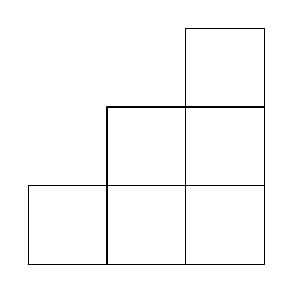
\begin{tikzpicture}[line join = round, line cap = round,>=stealth,font=\footnotesize,scale=1]
			\draw (0,0) -- (3,0) -- (3,3) -- (2,3) -- (2,2) -- (1,2) -- (1,1) -- (0,1) -- (0,0) (2,0) -- (2,2) -- (3,2) (1,0) -- (1,1) -- (3,1);
		\end{tikzpicture}
	}
	\par \shortans{$36$}
	\loigiai
	{
		Tổng ba số nhỏ nhất ở hàng cuối là $2+3+4=9$ nên số ở hàng đầu tiên chỉ có thể là $9$, $10$, $11$.
		\begin{itemize}
			\item Nếu tổng ở mỗi hàng là $9$ thì ba số ở hàng cuối là $2$, $3$, $4$. Số ở hàng trên cùng là $9$. Tổng $2$ số ở hàng thứ $2$ là $9=8+1=7+2=6+3=5+4$ (đều không thoả mãn).
			\item Nếu tổng ở mỗi hàng là $10$ thì hàng trên cùng là số $10$. Ba số ở hàng cuối chỉ có thể là $2$, $3$, $5$. Do đó $2$ chữ số ở hàng giữa chỉ có thể là $4$, $6$ (các trường hợp $(2;8)$, $(3;7)$ đều không thoả mãn).
			\item Nếu tổng ở mỗi hàng là $11$ thì hàng trên cùng là số $11$. Ba số ở hàng cuối chỉ có thể là $(2;3;6)$ hoặc $(2;4;5)$.
			\begin{itemize}
				\item Ba số ở hàng cuối là $(2;3;6)$ thì $11=9+2=8+3=7+4=6+5$ nên $2$ số ở hàng giữa chỉ có thể là $(4;7)$.
				\item Ba số ở hàng cuối là $(2;4;5)$ thì $11=9+2=8+3=7+4=6+5$ nên $2$ số ở hàng giữa chỉ có thể là $(8;3)$.
			\end{itemize}
			Vậy chỉ có $3$ cách chọn sáu số từ $10$ số $2;3;\ldots;11$ thoả mãn yêu cầu bài toán.
		\end{itemize}
		Số cách điền $6$ số vào các ô là $1!\cdot 2!\cdot 3!=12$.\\
		Vậy số cách chọn ra $6$ số từ $10$ số và điền vào các ô vuông là $3\cdot 12=36$ (cách).
	}
\end{ex}
\Closesolutionfile{ans}

%\indapan{6}{ans/ans-26-2--SoGDThaiNguyen-L1-LC}
%\indapan{4}{ans/ans-26-2--SoGDThaiNguyen-L1-DS}
%\indapan{6}{ans/ans-26-2--SoGDThaiNguyen-L1-KQ}